\chapter{SLAM Framework}
\label{chapter:ScaViSLAM}

This chapter will describe the underlying SLAM system used for this work, \\ \mbox{ScaViSLAM}\cite{strasdat_11}.  \mbox{ScaViSLAM}, (Scalable Visual SLAM) is a stereo visual SLAM system designed to do online constant time SLAM.  ScaViSLAM is an existing, functional system that is open source software publicly available under the GNU Lesser General Public License.

ScaViSLAM achieves constant time SLAM by using a SLAM graph, and rather than optimizing over the whole graph, it optimizes using a 'double window' approach to select which parts of the graph to optimize.  This consists of an 'inner window', where a bundle adjustment over all poses and landmarks is performed, and an 'outer window', where an optimization over only keyframes and keyframe-keyframe edges is done. The outer and inner window are dynamically calculated by the algorithm during operation.  This double-window approach allows for only a subsection of the graph to be optimized each step, thus solving in constant time, whilst still allowing for the entire graph to remain consistent.

The inner workings of ScaViSLAM may be broken up into three different modules, each of which runs in a separate thread; stereo frontend, SLAM graph backend and place recognition. These modules will be discussed here. In addition to the modules, the operation of the SLAM graph will be expanded on, as not only is this the main novelty of ScaViSLAM, but is also very important in the context of the contribution of this work. The main interface between the pipeline presented in this work and ScaViSLAM is by adding information to the SLAM graph.

\begin{figure}[h!]
  \centering
    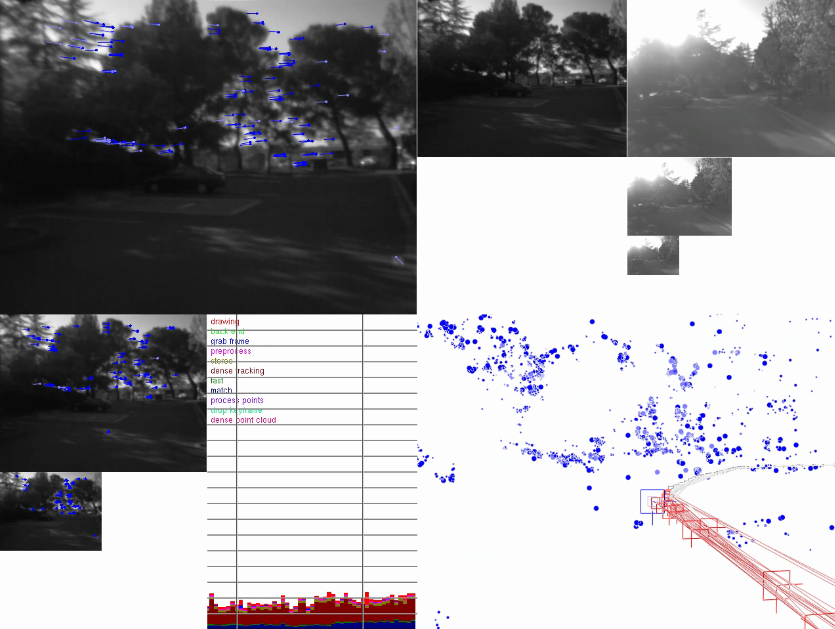
\includegraphics[width=0.8\textwidth]{chapters/images/scavislam_gui}
    \caption{ScaViSLAM visualization.  The left shows tracking against the current keyframe using an image pyramid.  On the right is a visualization of the SLAM graph}
  \label{fig:scavislam_gui}
\end{figure}

\section{Frontend}
\label{sec:scavislam_frontend}

The frontend is responsible for calculating visual odometry.  It also finds landmarks and estimates their 3D positions using stereo information.  Another responsibility is creating new keyframes, containing all the logic for when to generate a new keyframe or switch to an old one. 

\subsection{Visual Odometry}

To calculate an initial transformation between frames, first a disparity image is calculated using dense stereo matching\cite{dense_match}, then dense stereo tracking is performed.  Both of these operations are done on the GPU.  After an initial transformation has been estimated, landmarks are matched used guided BRIEF\cite{brief_10} at FAST\cite{rosten_06} corners locations.  Matching is done on multiple image pyramid levels to allow features of various scales. Selection of landmarks will be discussed in the following section.  Image patches of landmarks are warped into the current perspective by using the current transformation to improve matching. Having matched enough points against current and previous keyframes, a refined pose is calculated by minimising reprojection error over all point correspondences.

\subsection{Tracking points}

In an outdoor setting there are often many landmarks to track and therefore it is important to select reliable points to track in the interest of robustness and scalability.  Therefore the following criteria is applied:
\begin{itemize}
 \setlength{\itemsep}{0cm}%
 \setlength{\parskip}{0cm}%
 \item Visible from either current keyframe or adjacent keyframe
 \item Reprojection error is within a threshold
 \item Not too far
 \item Not too close
 \item Change in viewing angle between frames not too large
\end{itemize}

\subsection{Creates Keyframes}

New keyframes are added either when the number of shared observations drops below a certain threshold, or a certain metric distance from the last keyframe has been passed.  This ensures good interconnectivity between all keyframes.  As new keyframes, landmarks and landmark observations are created, these are passed to the backend to be integrated into the graph.

\section{Backend}
\label{sec:scavislam_backend}

The backend is responsible for maintaining the entire SLAM graph, and thus holds internally its own representation of the whole graph.  It provides interfaces for other modules to add information to the graph, such as the frontend with new keyframes or the place recognizer with new large loop closures. It is also responsible for solving the graph, in this case by using the g2o library\cite{g2o}. As the graph is designed to run in constant time, the backend has been designed to execute at a relatively fast rate so that the graph may be constantly solved during operation.

%\subsection{Contains the entire graph (not in g2o format)}
%\subsection{Performs some bundle adjustment}
%\subsection{Acts as a wrapper for g2o}

The backend runs optimization whenever new information is added to the graph.  It contains data structures to represent all keyframes, keyframe edges, landmarks and landmark observations.  For each optimization, only the necessary keyframes and edges are copied into the optimizer.  After optimization has been performed, the optimized vertices are copied back to ScaViSLAM representation of the graph, and the optimizer object is discarded.

\section{Place Recognition}
\label{sec:scavislam_place_recog}

The place recognition module is responsible for detecting 'large loop closures' between keyframes.

\subsection{Bag of words}

One solution to finding large loop closures between keyframes would be to compare every keyframe with every other keyframe generated.  However this would result in a time complexity of $O(n^2)$ for $n$ frames.  This does clearly not scale well to large maps.

A better solution is to use an appearance based place recognition algorithm, which given a collection of images of various locations, attempts to match a query frame to an existing location, without searching through the entire image space.  For more on place recognition, see Section \ref{sec:bag_of_words}.  In ScaViSLAM the bag of words approach was employed.

The existing implementation of bag of words in ScaViSLAM generates potential matches by determining a score for location pairs.  If the score is above a certain threshold, this frame pair will be identified as a potential loop closure and then tested with a geometry check.

\subsection{Geometry check}
\label{subsec:geometry_check}

The geometry check serves two purposes; one is to filter out false positives as generated by the place recognition module.  The bag of words implementation in ScaViSLAM is rather simplistic and as a result outputs many false positives.  The second purpose is to generate an estimation of the pose between keyframes so it may be integrated into the SLAM graph.  

To do this check, features are extracted from both frames and projected to 3D points using stereo information.  3D-3D correspondences are obtained from feature matching between frames and a three point 6 DoF solver\cite{umeyama} coupled with RANSAC is used to find an optimal transformation.  If enough inliers are returned then the edge may be added to the graph.  The number of inliers may be used to weight the strength of this pose-pose graph constraint.

\section{ScaViSLAM Graph}
\label{sec:scavislam_graph}

\subsection{Graph description}

The specific SLAM graph implementation will be covered here.  The graph may be split up into two parts, an inner and an outer window.  These will be described first separately, and followed by how they work together.

The SLAM solver used by ScaViSLAM is g2o.  g2o is c++ framework for solving optimization of non-linear least squares problems that can be described by a hyper-graph.  (Section \ref{subsec:graph_slam})

\subsubsection{Inner Window}

The inner window of the graph does a bundle adjustment over keyframe poses as well as landmark positions, using edges of landmark observations.  See fig \ref{fig:inner_window}.

\begin{figure}[h!]
  \centering
    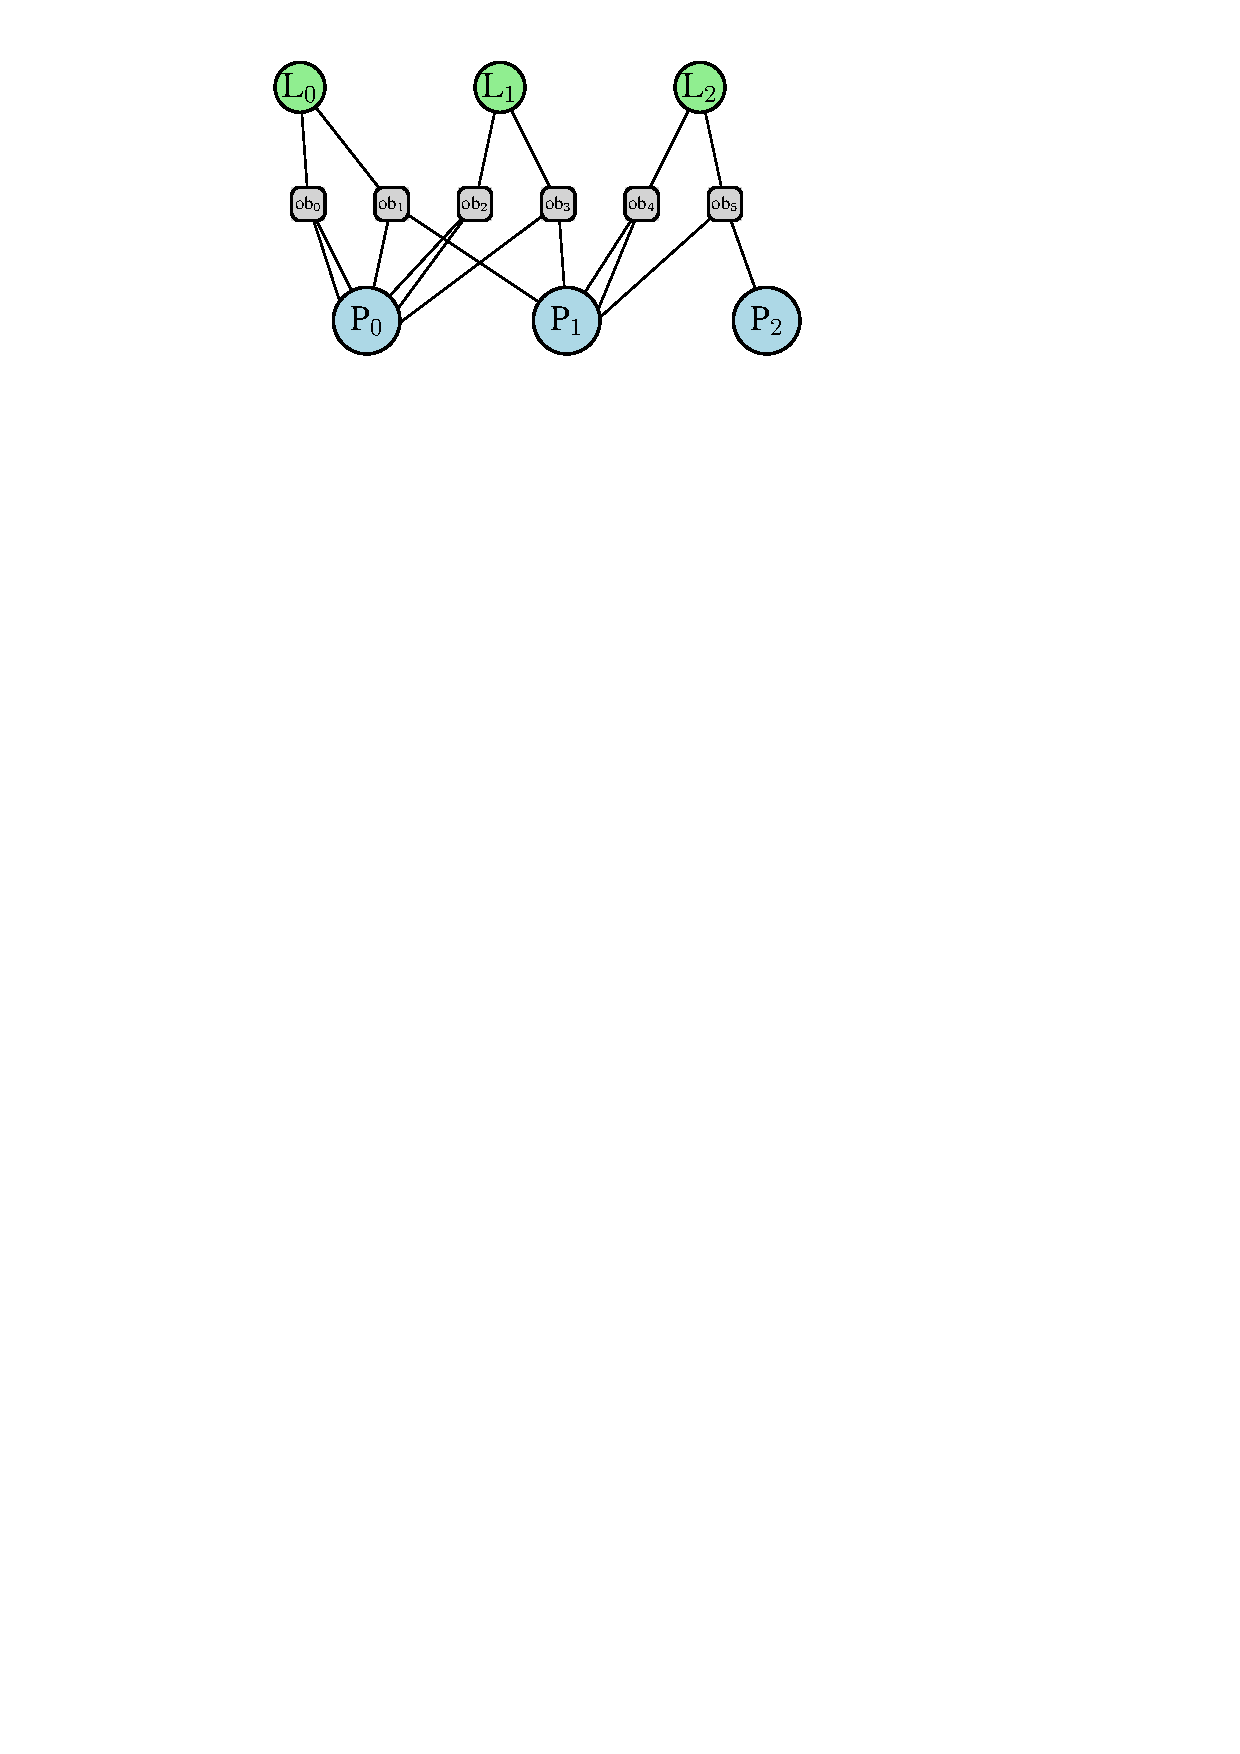
\includegraphics[width=0.6\textwidth]{chapters/images/inner_window}
  \caption{Simplified graph representation of the inner window.  $\bv P_i$ are poses, $\bv L_i$ are landmarks, and $\bv {ob}_i$ are observation edges}
  \label{fig:inner_window}
\end{figure}

$\bv P_i$ represent 3D camera poses of keyframes $SE(3)$.  $\bv L_i$ is a landmark position and is represented as a 3D point $\mathbb{R}^3$ in the frame of the keyframe where it was first recorded.  This will be referred to as that point's anchor keyframe.  It it important to note that the landmark is not represented in world coordinates, and therefore its position is also dependent on the anchor keyframe vertex state.

$\bv {ob}_i$ represents the observations of landmarks.  They are multi edges between the landmark, the anchor keyframe and the pose where it is observed from.  This also means the first observation of a landmark will contain two connections to the anchor keyframe. The error function in this case is a reprojection error and is calculated as follows;

\begin{align}
 \bv e = \bv z_O - \hat{\bv z}( ^{O}\bv T_W \ ^W \bv T_{A} \ \bv L_{A})
\end{align}

$\bv z_O$ is the edge constraint stored as the pixel coordinates of the landmark in left and right frame seen from the observation  frame. $\bv L_{A}$ is the landmark in the anchor frame (landmark vertex).  $^W \bv T_{A}$ is the transformation from the anchor keyframe to world frame (anchor keyframe vertex), and $^{O}\bv T_w$ is the transformation from the world frame to the observation keyframe -  where this particular edge was recorded.  The $\hat{\bv z}$ function uses intrinsic camera calibration parameters and projects a 3D point into image pixel coordinates.

\subsection{Outer Window}

Unlike the bundle adjustment of the inner window, the outer window is a simple pose graph optimization.  It contains keyframe poses as in the inner window, and keyframe edges, which describe a transformation from one keyframe to another.  They are binary edges, only relating two poses at most.  The error function is then defined as follows:

\begin{align}
 v_{AB} &=  \log(^{W}\bv T_{A} \ ^{A} \bv T_{B} \ ^{B} \bv T_{W}) \\
 \bv e &= v_{AB}^T \ \Lambda_{AB} \ v_{AB}
\end{align}

\begin{figure}[h!]
  \centering
    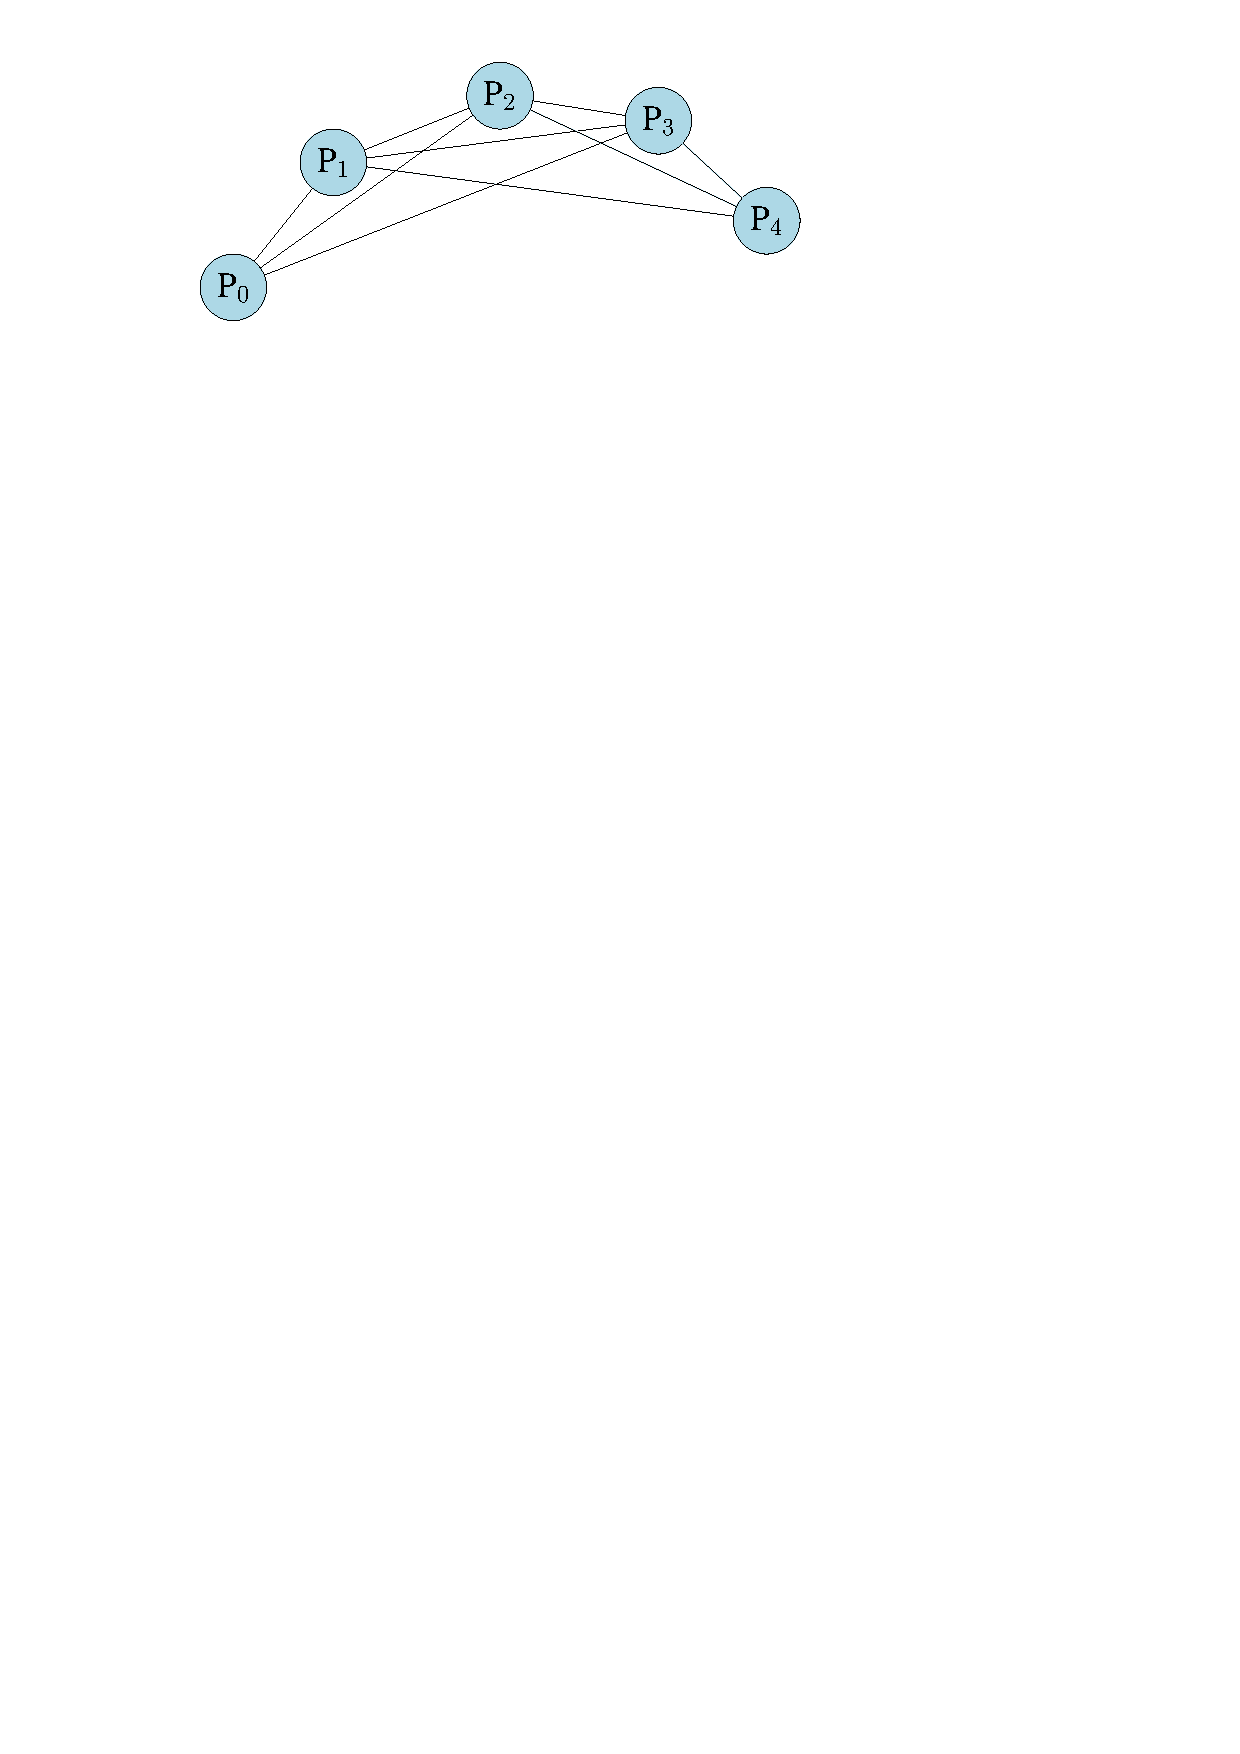
\includegraphics[width=0.6\textwidth]{chapters/images/outer_window}
  \caption{Simplified graph representation of the outer window.  $\bv P_i$ are poses, connecting lines are SE(3) edges}
  \label{fig:outer_window}
\end{figure}

$^{W}\bv T_{A}$ and $^{B} \bv T_{W}$ are obtained from the vertex states, while $^{A} \bv T_{B}$ is the edge measurement.  The logarithmic function is a lie group mapping that maps the transformation to a 6D vector. (Section \ref{sec:lie_group})  $\Lambda$ is the information matrix of the edge.  The rotational part is estimated using the number of shared observations.  The translational part is estimated using the average scene depth, that is, if all points are far away, the depth estimation will be poor.

\subsection{Window selection}

The idea of the double window approach is to obtain high accuracy locally by using bundle adjustment, whilst still having a globally consistent graph that optimizes in real time.  This is achieved by 'marginalizing' the bundle adjustment to a pose graph that can optimize much faster and thus allow optimization over a large map.

To calculate the double window, the current frame is first selected, and then a uniform cost search is performed over all neighbours of the current frame, selecting the frames with the highest number of shared observations first. The size of the inner window and outer window are parameterizable, denoted $W_1$ and $W_2$. The search is performed until $W_1$ + $W_2$ vertices are found, adding the first $W_1$ frames to the inner window and the rest to the outer window. Then all points visible from inner window frames are added to the inner window.  

\begin{figure}[h!]
  \centering
    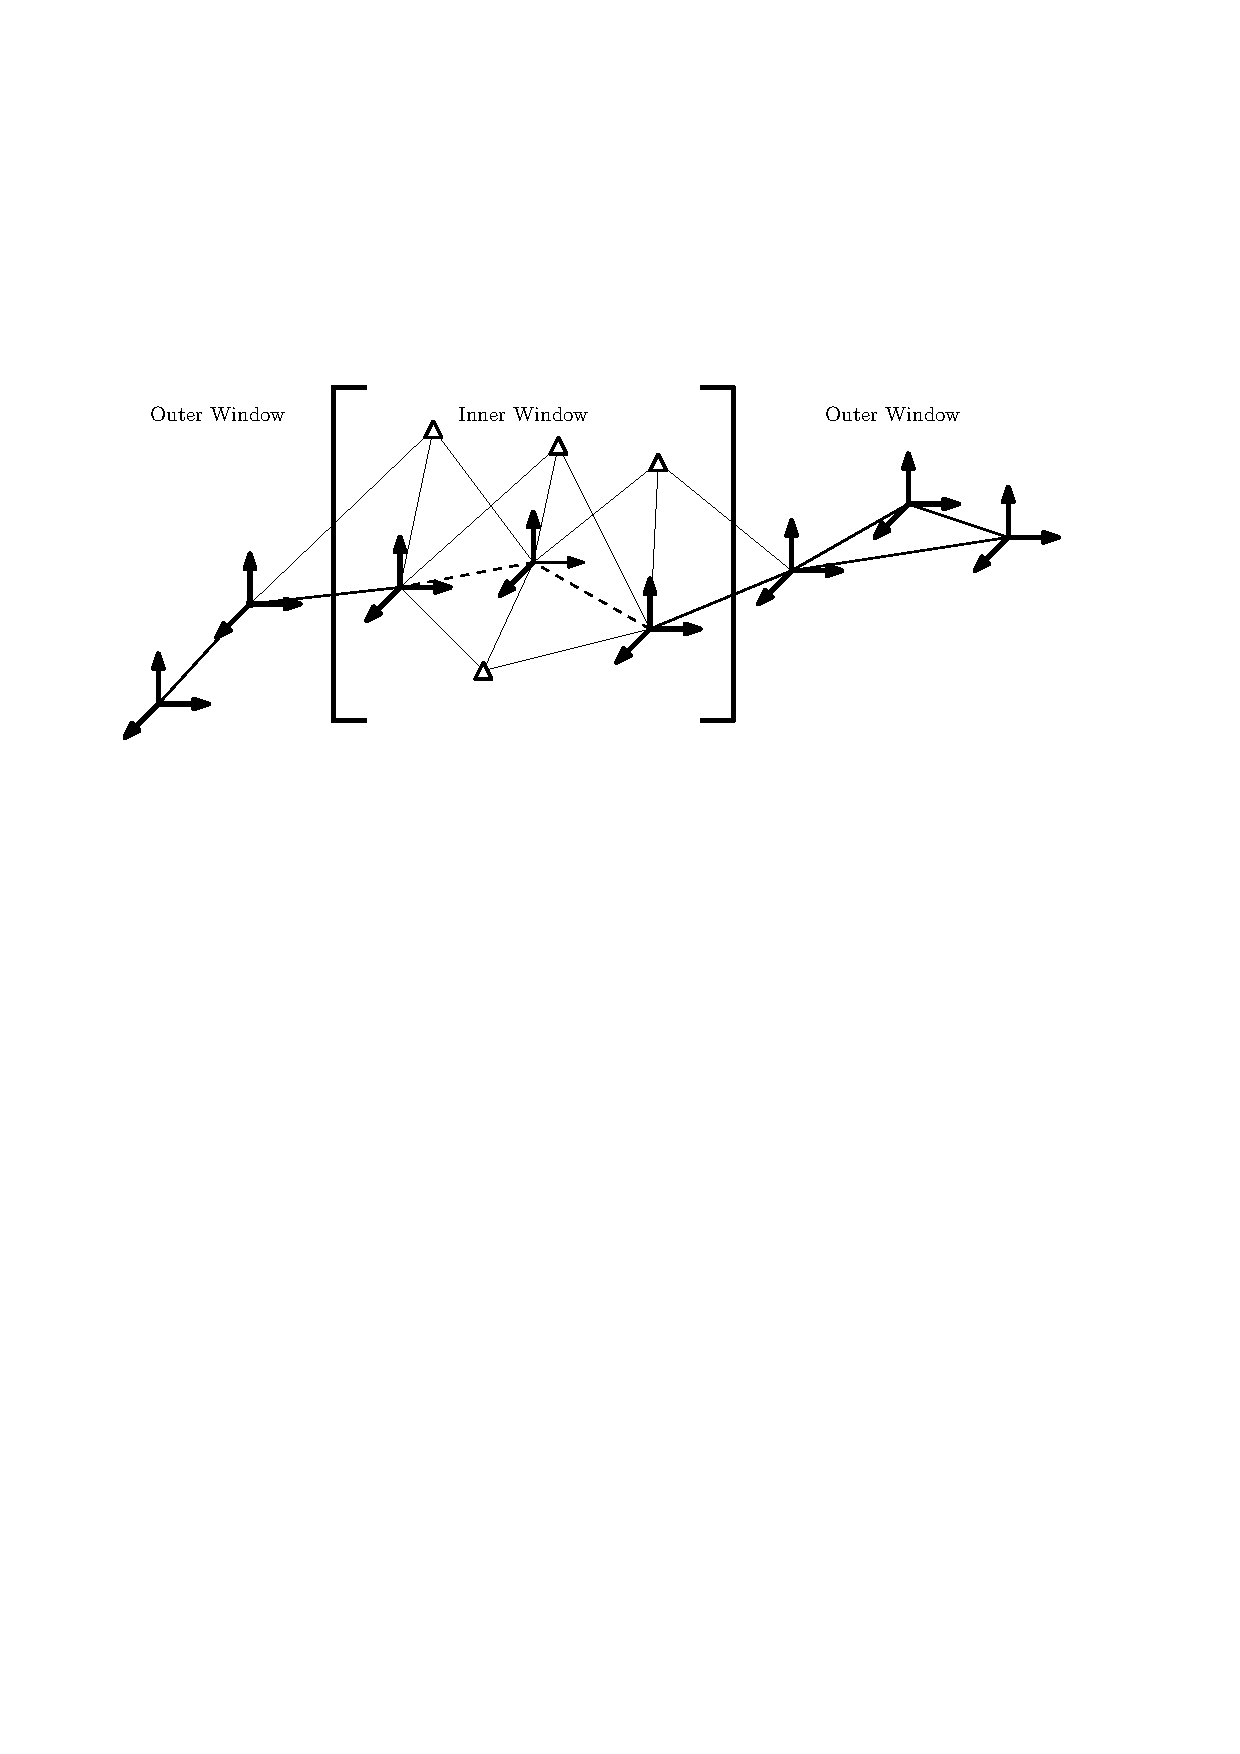
\includegraphics[width=1.0\textwidth]{chapters/images/double_win}
  \caption{Double Window}
  \label{fig:double_window}
\end{figure}

All of the non border poses in the inner window have only point-pose constraints, the border poses have both pose-pose constraints and point-pose constraints, and the rest of the outer window has only pose-pose constraints.  This is illustrated in Fig. \ref{fig:double_window}.  

This graph design allows for the inner window to calculate locally very accurate poses, whilst globally remaining consistent and still run in real time.

\subsubsection{Readjustment of double window after a loop closure}
As mentioned in section \ref{subsec:geometry_check}, pose-pose constraints are added to the graph in the event of a large loop closure. Due to the double window approach, simply adding the pose constraint will not close the loop, as pose edges are not considered in the inner window.  Instead, the current keyframe is initialized to its new position based on the loop closure edge, and then shared observations between current and old keyframes are searched for.  If successful, the landmarks are merged and the old keyframes are added to the inner window.  Optimization is then executed with the new double window.  The inner window pulls old and new keyframes together, while the outer window propagates error throughout the rest of the graph.


%\begin{itemize}
%\itemsep0em
 %\item SE(3) keyframes
 %\item SE(3) keyframe-keyframe edge
 %\item 3D Vector Landmark
 %\item 3D Vector UVU reprojection keyframe-landmark edge
%\end{itemize}
%
%\subsection{Double Window Graph Optimization}
%\begin{itemize}
%\itemsep0em
 %\item B.A. inner window
 %\item Pose-Pose outer window
 %\item metrics to define windows
 %\item ensures constant graph optimize time (novel from this approach)
%\end{itemize}
